\section{Thursday June 4 2020}
    \subsection*{Using Right Python Path and Modules}
        which python returns /apps/bin/python\\
        need to explicitly use /usr/bin/python2 to get htcondor module to work. I tried changing what "python2" does in bashrc but was getting error messages\\
        /usr/bin/python2 -- this works\\
        /usr/bin/python3 -- no module named 'pytz' (needed for utils/utils.unixtimeconvert()\\
        python2 -- no module named "htcondor"\\
        python3 -- no module named "htcondor"\\

    \subsection*{gemc-jsonify footer issue}
        \begin{figure}[H]
        \centering
        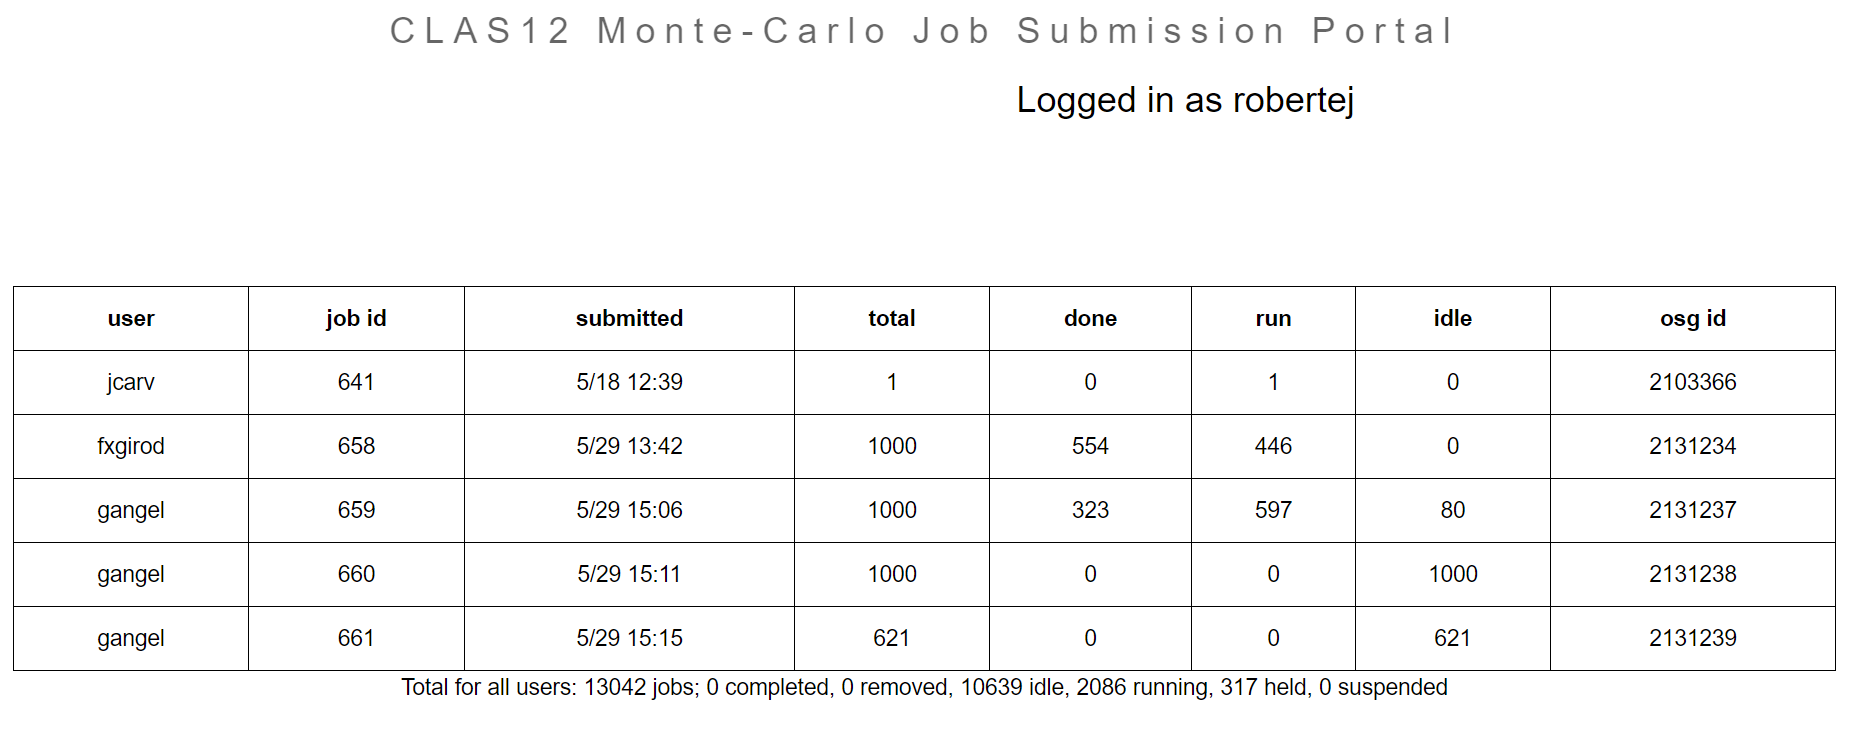
\includegraphics[scale=0.5]{Meetings/20200604/files/jobs-total.PNG}
        \caption{GEMC Web Portal Stats Table Example}
        \label{fig:my_label}
        \end{figure}

    
    Footer metadata - all jobs is for all jobs from JLab, not just CLAS12, this isn't very useful?
    
    \subsection*{Error Handling for when code breaks}
    Error handling: How do we want to handle this? Cant exactly print to screen. Want to send emails when things are breaking? Write to log? something else?
           
    
    \subsection*{Other}
    Are we still indending to put all hard coded variables into FS.py?\\
    Does an up to date Schema diagram for DB exist?\\
    any way to turn off bell in ssh terminal on ifarm? Can't edit /etc/config\\
    
    














